\documentclass{standalone}
% Preamble
\begin{document}

\subsection{Structure bloc-triangulaire et rang numérique de $B(1)$}

\begin{wrapfigure}{r}{8cm}
  \caption{matrice $B(1)$}
  \label{fig:B1}
  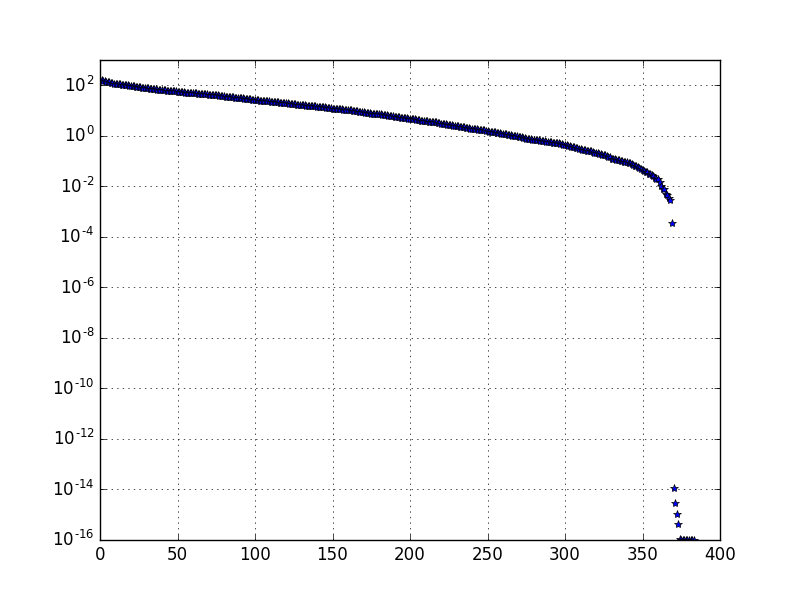
\includegraphics[width=8cm]{../png/bez_diag.png}
\end{wrapfigure}
Dans le processus de réduction, la première étape consiste à calculer le noyau de $B(1)$. Lorsque les coefficients des polynômes d'entrée sont entiers ou rationnels, ceci peut se faire de manière exacte au moyen d'un programme de calcul symbolique. La taille des entiers peut alors croître considérablement au cours des calculs et augmenter en conséquence le temps total de calcul et les besoins en mémoire du calculateur. Si par contre on veut effectuer l'ensemble des calculs en nombres flottants, ou si les coefficients d'entrée sont eux mêmes donnés sous forme numérique, alors on doit faire un calcul numérique du noyau. 
La méthode éprouvée pour cela, implémentée dans des packages d'algèbre linéaire numérique comme Matlab/Octave, Numpy ou Julia, est d'effectuer une factorisation QR ``rank revealing'' de $B(1)$, que nous appellerons factorisation QRP, c'est-à-dire accompagnée de pivots sur les colonnnes. L'expérience montre que cette approche est souvent efficace mais peut s'avérer délicate à mettre en oeuvre si la taille de la matrice augmente. 

Montrons le sur un exemple. Nous choisissons $n =\input{../txt/n.txt}$ et un système polynomial $f$ de multidegré $\input{../txt/deg.txt}$. Les coefficients, entiers, sont choisis aléatoirement suivant une loi gaussiènne (fonction ZZ.random\_element(0.5, distribution='gaussian') de Sage). La matrice de Bezout $B(1)$ est de taille $\input{../txt/Dx.txt}$ et possède une certaine structure, comme le montre la Figure \ref{fig:sparsity_B1}. Cependant il parait difficile d'exploiter cette structure pour le calcul numérique du rang de la matrice $B(1)$. On doit avoir recours à une méthode numérique générale, par exemple une factorisation SVD ou une factorisation QRP ``rank revealing''. Choisissons cette deuxième méthode. Les termes diagonaux du facteur triangulaire $R$ seront triés en ordre décroissant, comme le montre la Figure \ref{fig:diag_B1}. 
\begin{wrapfigure}{r}{8cm}
  \caption{$B(1)$ permutée sous forme bloc-triangulaire}
  \label{fig:B1_permuted}
  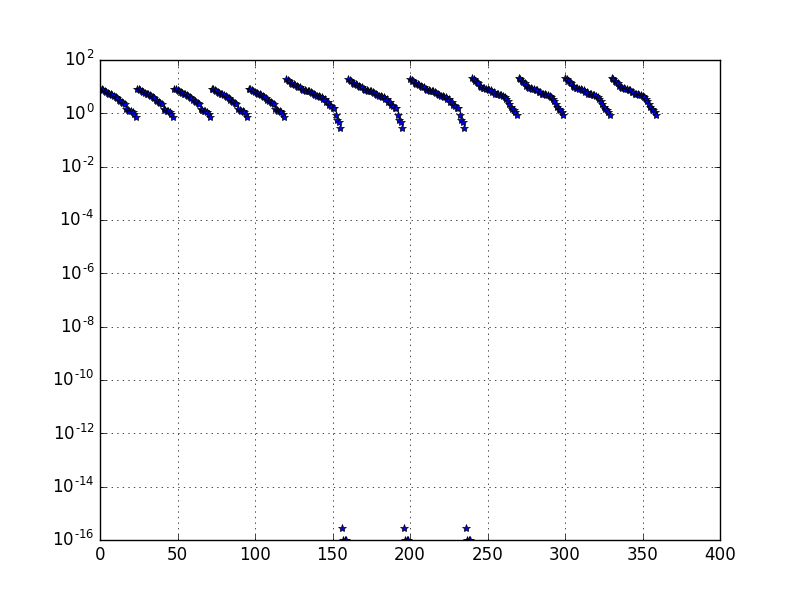
\includegraphics[width=8cm]{../png/beztri_diag.png}
\end{wrapfigure}

On s'aperçoit que les derniers termes non nuls décroissent vite, et qu'il peut devenir difficile de choisir un seuil au dessus duquel les termes diagonaux seront déclarés ``non nuls''. Le saut entre termes ``non-nuls'' et termes proches du epsilon machine a tendance à diminuer à mesure que la taille de la matrice augmente, ce qui rend le calcul du rang numérique difficile. Nous pouvons cependant améliorer, dans une certaine mesure, la situation précédente en exploitant une propriété de $B(1)$. En effet, en permutant lignes et colones de cette matrice d'une certaine façon, on peut arriver à une structure bloc-triangulaire de $B(1)$. En appliquant à la matrice une factorisation QRP bloc après bloc, les termes diagonaux vont alors décroitre uniquement à l'intérieur de chaque bloc. Le graphique ci dessous montre la nouvelle disposition des termes diagonaux à la fin de la factorisation QRP, en traitant les blocs l'un après l'autre. 
On voit que, malgré une décroissance rapide des termes diagonaux dans chaque bloc, la petite taille de ceux-ci permet au plus petit terme ``non-nul" d'être nettement grand que dans la factorisation QRP appliquée globalement à $B(1)$. Le calcul du rang numérique est facilité et l'on trouve ici un rang égal à $\input{../txt/dim0.txt}$, qui correspond au nombre de termes dans la figure ci-dessus. Enfin la dernière figure montre la distribution des termes diagonaux dans la matrice finale, une fois les réductions faites, comme expliqué dans la section \ref{sec:reduction_process}. On voit que la distribution des termes est toujours bonne. Le rang de la nouvelle matrice est $\input{../txt/dim.txt}$, c'est la dimension du quotient $A$, d'après la Conjecture~\ref{conjecture}.

\end{document}
%%%%%%%%%%%%%%%%%%%%%%%%%%%%%%%%%%%%%%%%%%%%%
Pour cet exemple, voici la table des termes de la diagonale entre les indices $294$ et $297$.
$$
\begin{array}{c|c}
 i & \vert R_{i,i}\vert \\
 \hline
 294  & 1e-4 \\
 295 & 1e-6 \\
 296 & 1e-11 \\
 297 & 1e-11 \\
\end{array}
$$
On constate qu'il est difficile, à partir de ces valeurs, de fixer un seuil en dessous duquel les termes peuvent être considérés comme négligeables. On aurait tendance à fixer naturellement le seuil entre les indices $295$ et $296$ ce qui donnerait $295$ comme rang numérique de $B(1)$. C'est la valeur fournie par les fonctions rank de numpy ou de Julia. Or $B(1)$ est une matrice à coefficients entiers et on peut donc calculer son rang exact au moyen d'un logiciel de calcul symbolique. Pour le logiciel Sage le rang de la matrice $B(1)$ vaut $296$, différent donc de la valeur obtenue par la factorisation numérique QRP précédente.
